% \documentclass[longbibliography,twocolumn,amsmath,amssymb,aps,nofootinbib]{revtex4-2}
\documentclass[longbibliography,amsmath,amssymb,aps,nofootinbib]{revtex4-2}

\usepackage{graphicx}
\usepackage{natbib}
\usepackage{amsmath}
\usepackage{longtable}
\usepackage{gensymb}
\usepackage{enumerate}
\usepackage{varwidth}
\usepackage{float}
\usepackage{nonfloat}
\usepackage{soul}
\usepackage{ulem}
% \usepackage{multicol}
% \usepackage{afterpage}
\usepackage[usenames, dvipsnames]{color}
\newcommand{\note}[1]{\noindent \textbf{\textit{\textcolor{Red}{#1}}}}

\newcommand\Ra{\mathrm{Ra}}
\newcommand\Pran{\mathrm{Pr}}
\newcommand\Rac{\mathrm{Ra}_{\mathrm{c}}}
\newcommand\Ek{\mathrm{Ek}}
\newcommand\Ro{\mathrm{Ro}}
\newcommand\Nu{\mathrm{Nu}}
\newcommand\Sc{\mathrm{Sc}}

\newcommand\eps{\varepsilon}
\renewcommand\L {\mathcal{L}}
\renewcommand{\citet}[1]{ref.~\cite{#1}}
\renewcommand{\Citet}[1]{Ref.~\cite{#1}}
\newcommand{\citets}[1]{refs.~\cite{#1}}
\newcommand{\Citets}[1]{Refs.~\cite{#1}}
\newcommand{\davg}[1]{\langle {#1} \rangle}
\newcommand{\n}{\\ \nonumber \\ }
\newcommand{\nn}{\nonumber}
\newcommand{\nnn}{\\ \nonumber \\ \nonumber}

\newcommand\ie{\textit{i.e.},~}
\newcommand\eg{\textit{e.g.},~}
\newcommand{\omicron}{o}

\newcommand{\pd}[1]{\partial_{#1}}
\renewcommand{\vec}[1]{\boldsymbol{#1}}
\newcommand{\M}[1]{\mathbf{#1}}
\newcommand{\grad}{\vec{\nabla}}
\newcommand{\cross}{\vec{\times}}
\newcommand{\laplacian}{\nabla^2}

\newcommand{\sump}[2]{\sideset{}{'}\sum_{{#1}=0}^{#2}}

\newcommand{\eq}[1]{(\ref{#1})}
\newcommand{\eqs}[2]{(\ref{#1})~\&~(\ref{#2})}
\newcommand{\eqss}[2]{(\ref{#1})--(\ref{#2})}

\newcommand{\Eq}[1]{Eq.~(\ref{#1})}
\newcommand{\Eqs}[2]{Eqs.~(\ref{#1})~\&~(\ref{#2})}
\newcommand{\Eqss}[2]{Eqs.~(\ref{#1})--(\ref{#2})}

\newcommand{\fig}[1]{Fig.~(\ref{#1})}
\newcommand{\figs}[2]{Figs.~(\ref{#1})~\&~(\ref{#2})}
\newcommand{\T}{{\cal T}}
\newcommand{\Z}{{\cal Z}}


\makeatletter
\let\Hy@backout\@gobble
\makeatother

\newcommand*{\GtrSim}{\smallrel\gtrsim}

\makeatletter
\newcommand*{\smallrel}[2][.8]{%
  \mathrel{\mathpalette{\smallrel@{#1}}{#2}}%
}
\newcommand*{\smallrel@}[3]{%
  % #1: scale factor
  % #2: math style
  % #3: symbol
  \sbox0{$#2\vcenter{}$}%
  \dimen@=\ht0 %
  \raise\dimen@\hbox{%
    \scalebox{#1}{%
      \raise-\dimen@\hbox{$#2#3\m@th$}%
    }%
  }%
}
\makeatother


\begin{document}

\title{Least-Squares Time Reversal of PDEs}

\author{Liam O'Connor$^{1,2}$}
\affiliation{%
$^1$Department of Engineering Sciences and Applied Mathematics, Northwestern University, Evanston, IL 60208 USA}
\affiliation{%
$^2$Center for Interdisciplinary Exploration and Research in Astrophysics, Northwestern University, Evanston, IL, 60201 USA}

\begin{abstract}
    abstract
\end{abstract}

\maketitle

\section{Introduction}
Rayleigh-B\'enard convection plays a foundational role in astrophysical and geophysical settings.
The resulting buoyancy-driven flows regulate heat transfer and generate large-scale vortices \cite{Couston}.
Turbulent convection, which is associated with large Rayleigh numbers $\Ra$, is difficult to simulate. 
State of the art simulations performed by \cite{Zhu_2018} have reached $\Ra \sim 10^{14}$ but estimates for the sun's convective zone and earth's interior are $\Ra \sim 10^{16}-10^{20}$ and $\Ra \sim 10^{20}-10^{30}$ respectively \cite{Ossendrijver,Gubbins_2001}. 

% \vspace{1cm}
% \textbf{Grad and Div}

% suppose $f(x, y, z):\mathbb{R}^3 \to \mathbb{R}$

% suppose $\vec{F}(x, y, z):\mathbb{R}^3 \to \mathbb{R}^3$
% \begin{align*}
%   \textbf{Gradient:}&\quad \grad f(x,y,z) \quad \longrightarrow \quad vector \\
%   \textbf{Divergence:}&\quad \grad \cdot \vec{F}(x,y,z) \quad \longrightarrow \quad scalar
% \end{align*}
% \vspace{1cm}

% \textbf{Navier-Stokes Equation}

% \begin{align*}
%   \intertext{Newton's 2nd law:}
%   \vec{F} &= m\vec{a} \\
%   &= \frac{d}{dt} [m\vec{u}]
% \end{align*}

% \begin{align*}
%   \intertext{Consider a velocity $\vec{u}(x, y, t)$}
%   \textbf{Conservation of momentum:} &\quad \partial_t \vec{u} = - \vec{u} \cdot \grad\vec{u} - \grad p + \nu \grad^2 \vec{u} + \vec{F} \tag{1}\\
%   \text{Inertial Term:} &\quad \vec{u}\cdot\grad\vec{u} \\
%   \text{Pressure Gradient Term:} &\quad \grad p \\
%   \text{Diffusive (Friction) Term:} &\quad \nu \laplacian \vec{u} \\
%   \text{Body Force:} &\quad \vec{F} \\
%   &\; \\
%   \textbf{Conservation of mass:} &\quad \grad \cdot \vec{u} = 0 \tag{2}\\
%   p(x, y, t) &= f(t) \; [\sum \sum (a_n\sin(nx)b_m\sin(my))]
% \end{align*}

\clearpage
\section{Generalized Problem Setup}
We define a generalized solution state vector $\bar{X}$ and associated initial value problem
\begin{align}
  \mathcal{F}[\bar{X}] &\equiv \partial_t \bar{X} + L . \bar{X} + N[\bar{X}, \bar{X}] = 0. \label{genpde}
  \intertext{Given a target end state $\bar{X}(\vec{x}, T)$, our aim is to recover the associated initial condition $\bar{X}(\vec{x}, 0)$.  
  This is realized by performing gradient-based minimization of the functional}
  H[X, \bar{X}] &= \frac{1}{2}\davg{|X(\vec{x}, T) - \bar{X}(\vec{x}, T)|^2} = \frac{1}{2}\davg{X'^2(\vec{x}, T)} \label{Hdef}, 
\end{align}
with respect to $X(\vec{x}, 0)$, where $X(\vec{x}, t)$ obeys (\ref{genpde}). The operator $\davg{\cdot}$ denotes the domain-integrated average and the quantity $X'(\vec{x}, t) \equiv X(\vec{x}, t) - \bar{X}(\vec{x}, t)$. For the remainder of this paper, symbols with overbars (such as $\bar{X}(\vec{x}, T)$) will be used to denote the target solution, while their corresponding unannotated symbols (such as $X(\vec{x}, T)$) play the role of optimization parameters.

The Lagrangian associated with our initial value problem is given by
\begin{align*}
  \mathcal{L} &= \int_0^T \davg{\chi \cdot \mathcal{F}[X]} dt + H[X, \bar{X}].
  \intertext{Where $\chi(\vec{x}, T)$ is the Lagrangian Multiplier corresponding to $X(\vec{x}, T)$. Equating} \frac{\delta\L}{\delta X} &= 0 \quad \text{and} \quad \frac{\delta\L}{\delta \chi} = 0 
  \intertext{yields the original and adjoint systems} 
  \mathcal{F}[X] &= 0 \quad \text{and} \quad \mathcal{F}^{\dagger}[\chi, X] = 0 \intertext{respectively. At some particular guess $X^n(\vec{x}, 0)$, we compute the functional derivative}
  \frac{\delta\L}{\delta X^n(\vec{x}, 0)} &= -\chi^n(\vec{x}, 0)
  \intertext{to determine the direction of steepest descent. Naive gradient-descent can then be performed by computing an updated guess}
  X^{n+1}(\vec{x}, 0) &= X^n(\vec{x}, 0) + \varepsilon \chi^n(\vec{x}, 0)
  \intertext{where $\varepsilon$ is the step size.}
\end{align*}
In addition to this algorithm, more advanced gradient-based optimization techniques such as conjugate gradient and BFGS have been employed in conjunction with adjoint-looping to improve performance and accelerate convergence.
In the context of our time-inversion optimization problem, such techniques traverse the space of possible initial conditions $X(\vec{x}, 0)$ by relying on local information pertaining to the objective functional $H$ and its functional derivative $\frac{\delta H}{\delta X(\vec{x}, 0)}$. 
For this reason, the focus of our investigation is largely centered around the objective functional's dependence on the initial condition.
More specifically, we study the levelsets of the objective functional because these surfaces characterize the directions of steepest descent at any arbitrary point in the space of initial conditions.
In doing so, we highlight the challenges and deficits associated with using the least squares functional (\ref{Hdef}) to recover the initial condition $\bar{X}(\vec{x}, 0)$ belonging to a target end state $\bar{X}(\vec{x}, T)$.


% Here I'll present a generalized PDE which we want to invert along with a bunch of notation. We'll define our target simulation, least-squares objective, and cite examples where the adjoint looping method has been successfully applied to inverse problems. We'll conclude this discussion by stressing the important of the objective function's shape in ``initial condition space'', because ultimately this is what curtails our gradient-based inversion technique.

\section{Preliminary Analysis}
\subsection{Linearity and Reversiblity}
In this section, we study linear initial value problems which do not include the nonlinear term in (\ref{genpde}), i.e. $N[X, X] = N[\bar{X}, \bar{X}] = 0$. Therefore $\mathcal{F}[X'] = \mathcal{F}[X] - \mathcal{F}[\bar{X}]$. 
In these special cases, the objective functional (\ref{Hdef}) depends only on the deviation's initial condition $X'(x, 0)$ about any arbitrary target $\bar{X}(x, 0)$.
For convenience when dealing with linear problems, we take $U(0) = U(T) = 0$ for all $x$.
In the following section, we demonstrate that the objective functionals of nonlinear systems with nonzero targets are directly influenced by one's choice of $U$.

Time-reversible wave equations of the form
\begin{align}
  \partial_t u &= \sum_{n \geq 1} c_n \partial^{2n - 1}_x u \label{waveeq}
  \intertext{are trivial cases of this optimization problem, because the quantity $\davg{u^2(x, t)}$ is conserved. 
  This implies that the objective functional's levelsets form sphere's in $u'$-space, because its value is given by $\davg{u'^2(T)} = \davg{u'^2(0)}$.
  The spatial derivatives in (\ref{waveeq}) are anti-self-adjoint (i.e. $L[u] = -L^{\dagger}[u]$), so the path of steepest descent is always in the radial derivation }
  \frac{\delta H}{\delta u(x, 0)} &= -u'(x, 0) \nonumber
  \intertext{In contrast, diffusive equations of the form}
  \partial_t u &= \sum_{n \geq 1} b_n \partial^{2n}_x u \label{waveeq}
  \intertext{do not conserve $\davg{u^2(x, t)}$, and consequently their objective functionals depend on $u'(x, 0)$'s \textit{direction} along with its magnitude. Suppose initial deviation can be written as}
  u'(x, 0) &= \sum_{k \geq 0} a_k e^{ikx}.
  \intertext{Let's just consider the diffusion equation ($n=1$). Then the end state is given by}
  u'(x, T) &= \sum_{k\geq 0} a_k \exp(ikx-Tb_1k^2) \label{diffsoln}\\
  \intertext{The nominal objective functional is given by}
  \davg{|u'(x, T)|^2} &= \pi \sum_{k \geq 0} \Big[a_k^2\exp\Big({-2T\sum_{n \geq 1} b_n k^{2n}  }\Big)\, \Big] \label{nomobjdiff}.
  \intertext{Equation (\ref{nomobjdiff}) gives us the elliptical heatmaps we observed previously.}
  \intertext{Let's take a second-order spatial derivative of (\ref{diffsoln})}
  \partial_x^2 u'(x, T) &= \pi \sum_{k\geq 0} -k^2 a_k^2 \exp(ikx-Tb_1k^2)\\
  \intertext{In general, applying a spatial derivative of order $2m$ to (\ref{diffsoln}), yields}
  \partial_x^{2m} u'(x, T) &= \pi \sum_{k\geq 0} (-k^2)^m a_k^2 \exp(ikx-Tb_1k^{2})\\
  \intertext{We can leverage this fact to construct an objective functional whose levelsets are spherical. Consider}
\end{align}
\begin{tiny}
\begin{align*}
  H[u'(T)] &= \davg{|u'(x, T) - (Tb_1)\partial_x^2 u'(x, T) + \frac{(Tb_1)^2}{2!}\partial_x^4 u'(x, T) - \frac{(Tb_1)^3}{3!}\partial_x^6 u'(x, T) ...|^2} \\
  &= \davg{\Big|\sum_{k\geq 0}a_k \exp(ikx-Tb_1k^2) + \sum_{k\geq 0}(Tb_1k^2)a_k \exp(ikx-Tb_1k^2) + \sum_{k\geq 0}\frac{(Tb_1k^2)^2}{2!}a_k \exp(ikx-Tb_1k^2) + \sum_{k\geq 0}\frac{(Tb_1k^2)^3}{3!}a_k \exp(ikx-Tb_1k^2) + ...\Big|^2} \\
  &= \davg{|\sum_{k\geq 0}\Big[a_k \exp(ikx-Tb_1k^2)\Big(1 + (Tb_1k^2) + \frac{(Tb_1k^2)^2}{2!} + \frac{(Tb_1k^2)^3}{3!} ...\Big)\Big]|^2} \\
  &= \davg{|\sum_{k\geq 0}\Big[ a_k \exp(ikx-Tb_1k^2) \Big( \exp(Tb_1k^2) \Big)\Big]|^2} \\
  &= \davg{|\sum_{k\geq 0}\Big[ a_k \exp(ikx)  \Big)\Big]|^2} \\
  &= \pi \sum_{k\geq 0} a_k^2
  % &= \pi \sum_{k \geq 0} \Big[\exp\Big({-2T\sum_{n \geq 1} b_n k^{2n}  }\Big)\, a_k^2\Big].
\end{align*}
\end{tiny}
That's gives us spherical objective levelsets. Notice what happens as we increment the number of terms in the above Taylor Series


\begin{figure*}[h]
  \centering
  \begin{tabular}{@{}c@{}}
      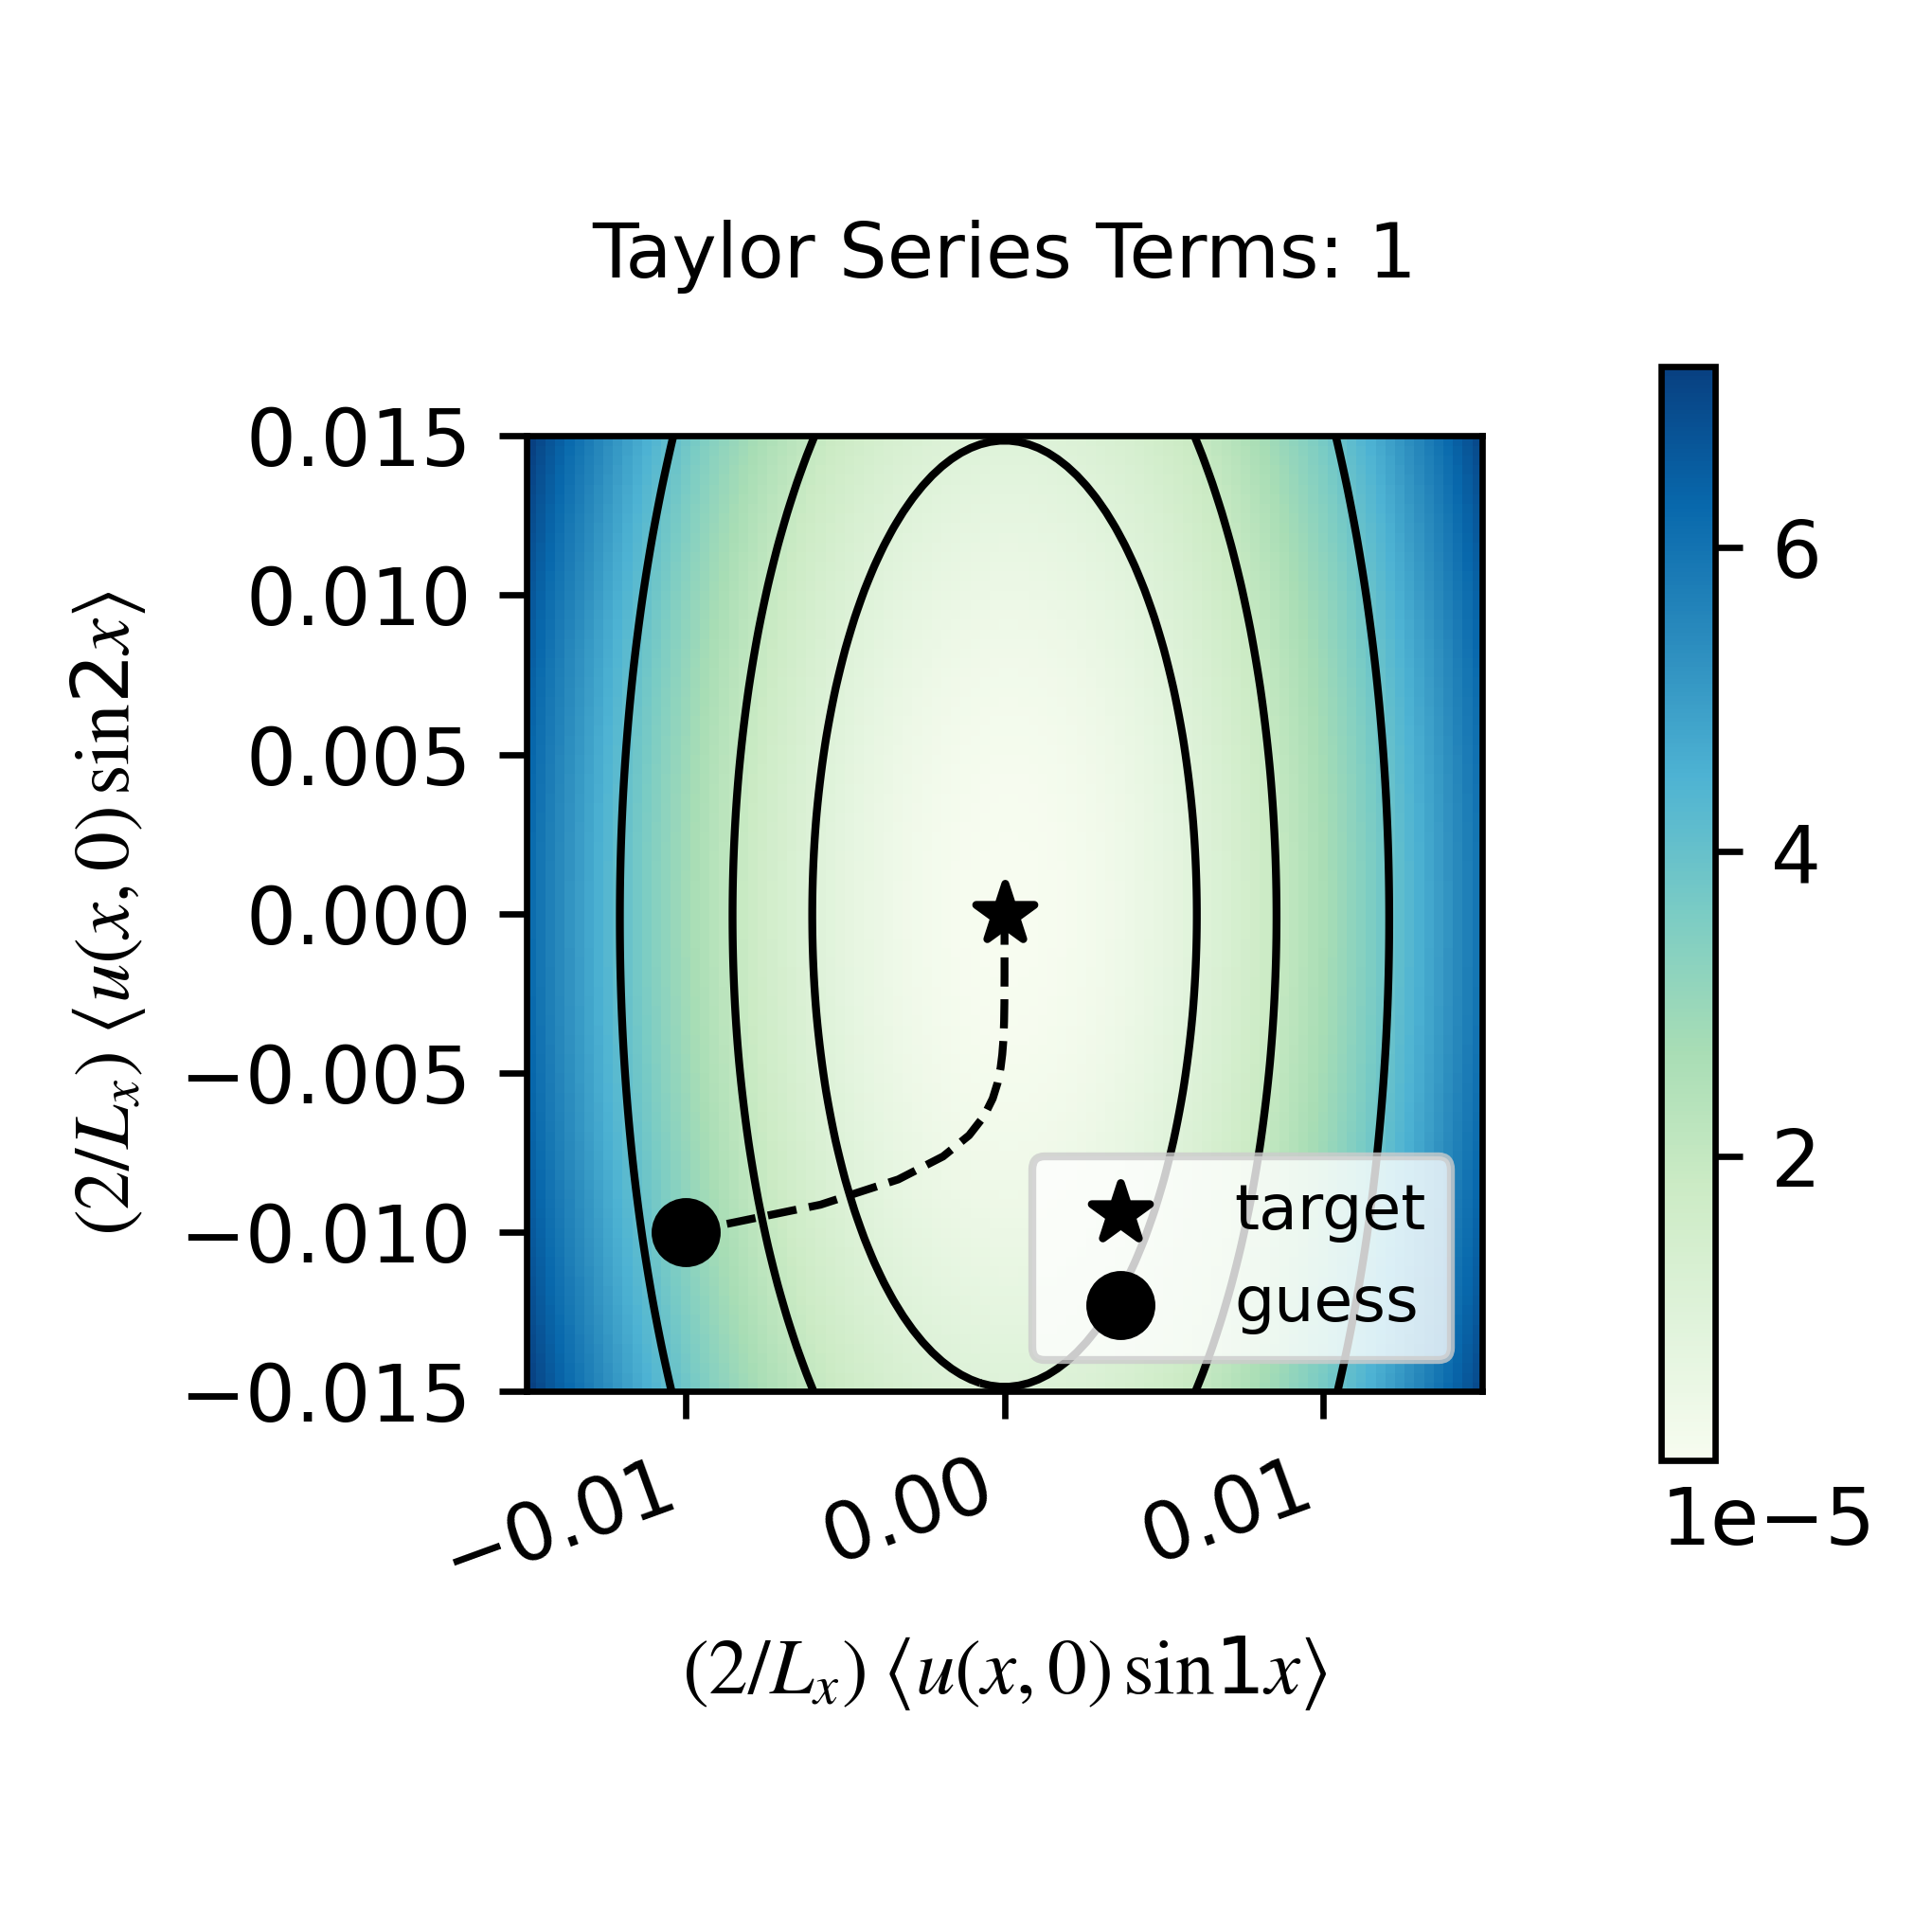
\includegraphics[width=3in]{SPHRtest_Nts1a0p3b0p0c0p0T1p0R0p015kt10p0kt20.png}
  \end{tabular}
  \begin{tabular}{@{}c@{}}
      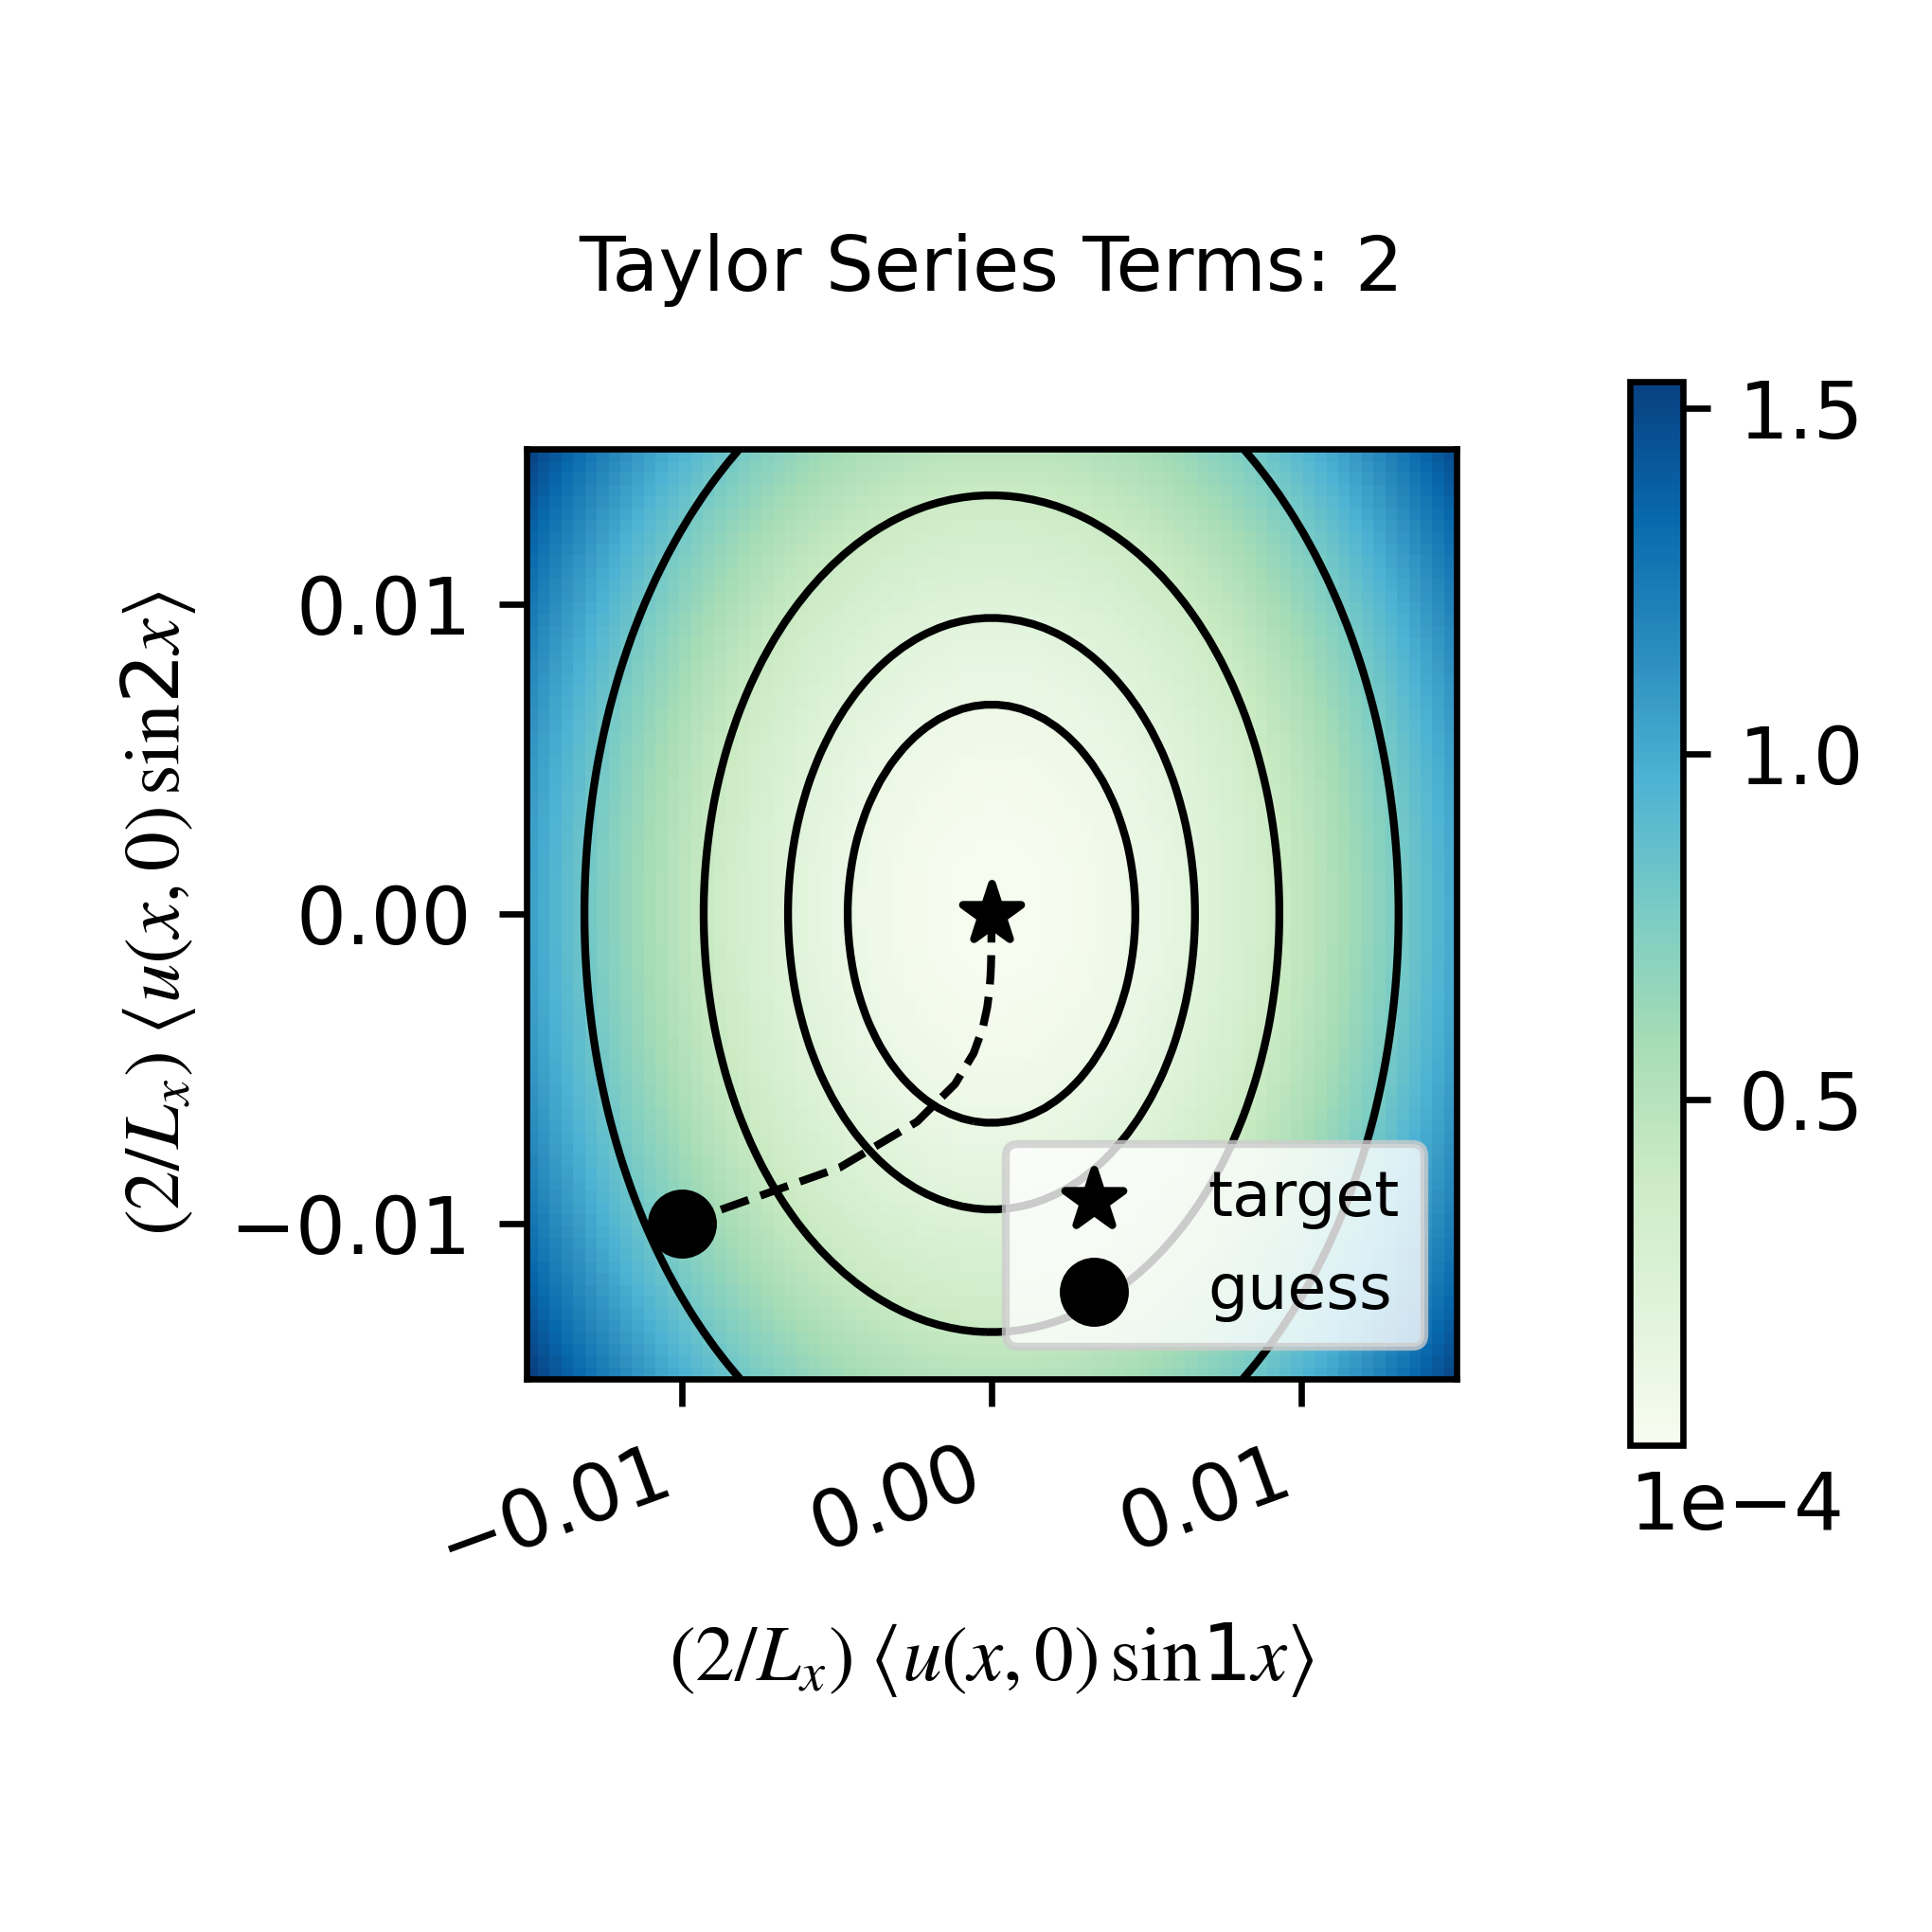
\includegraphics[width=3in]{SPHRtest_Nts2a0p3b0p0c0p0T1p0R0p015kt10p0kt20.png}
  \end{tabular}
  \begin{tabular}{@{}c@{}}
      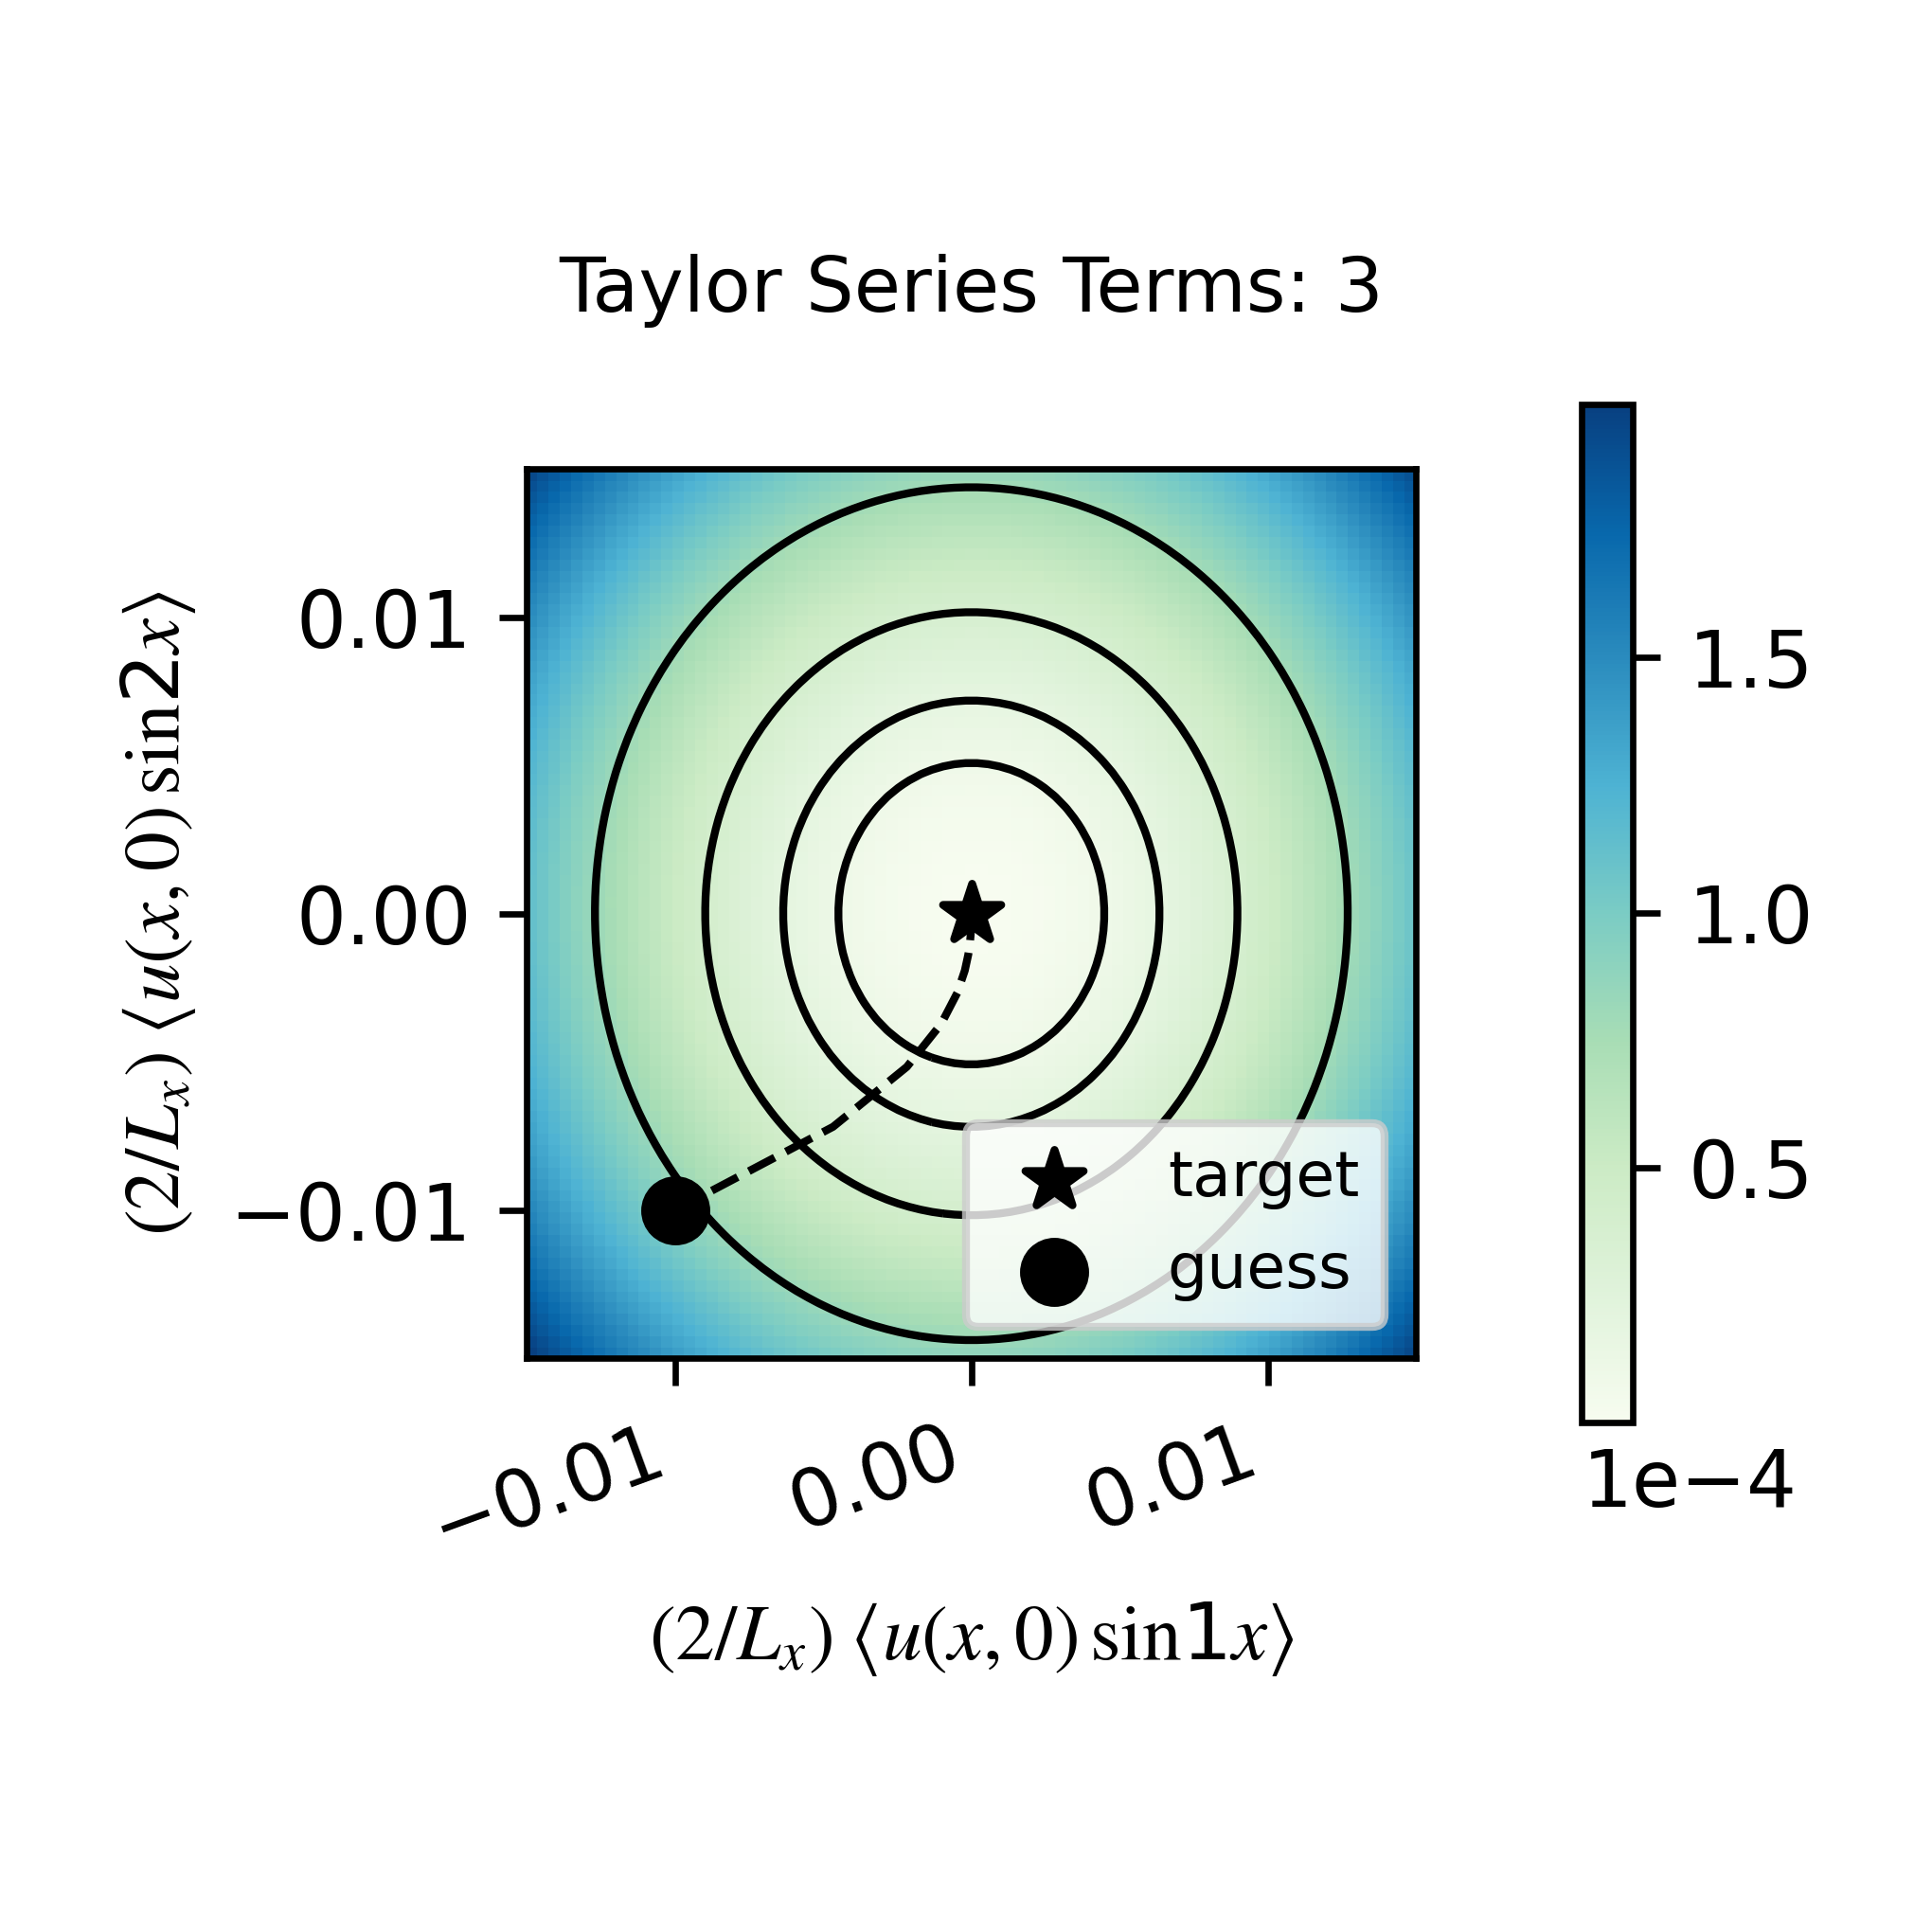
\includegraphics[width=3in]{SPHRtest_Nts3a0p3b0p0c0p0T1p0R0p015kt10p0kt20.png}
  \end{tabular}
  \begin{tabular}{@{}c@{}}
      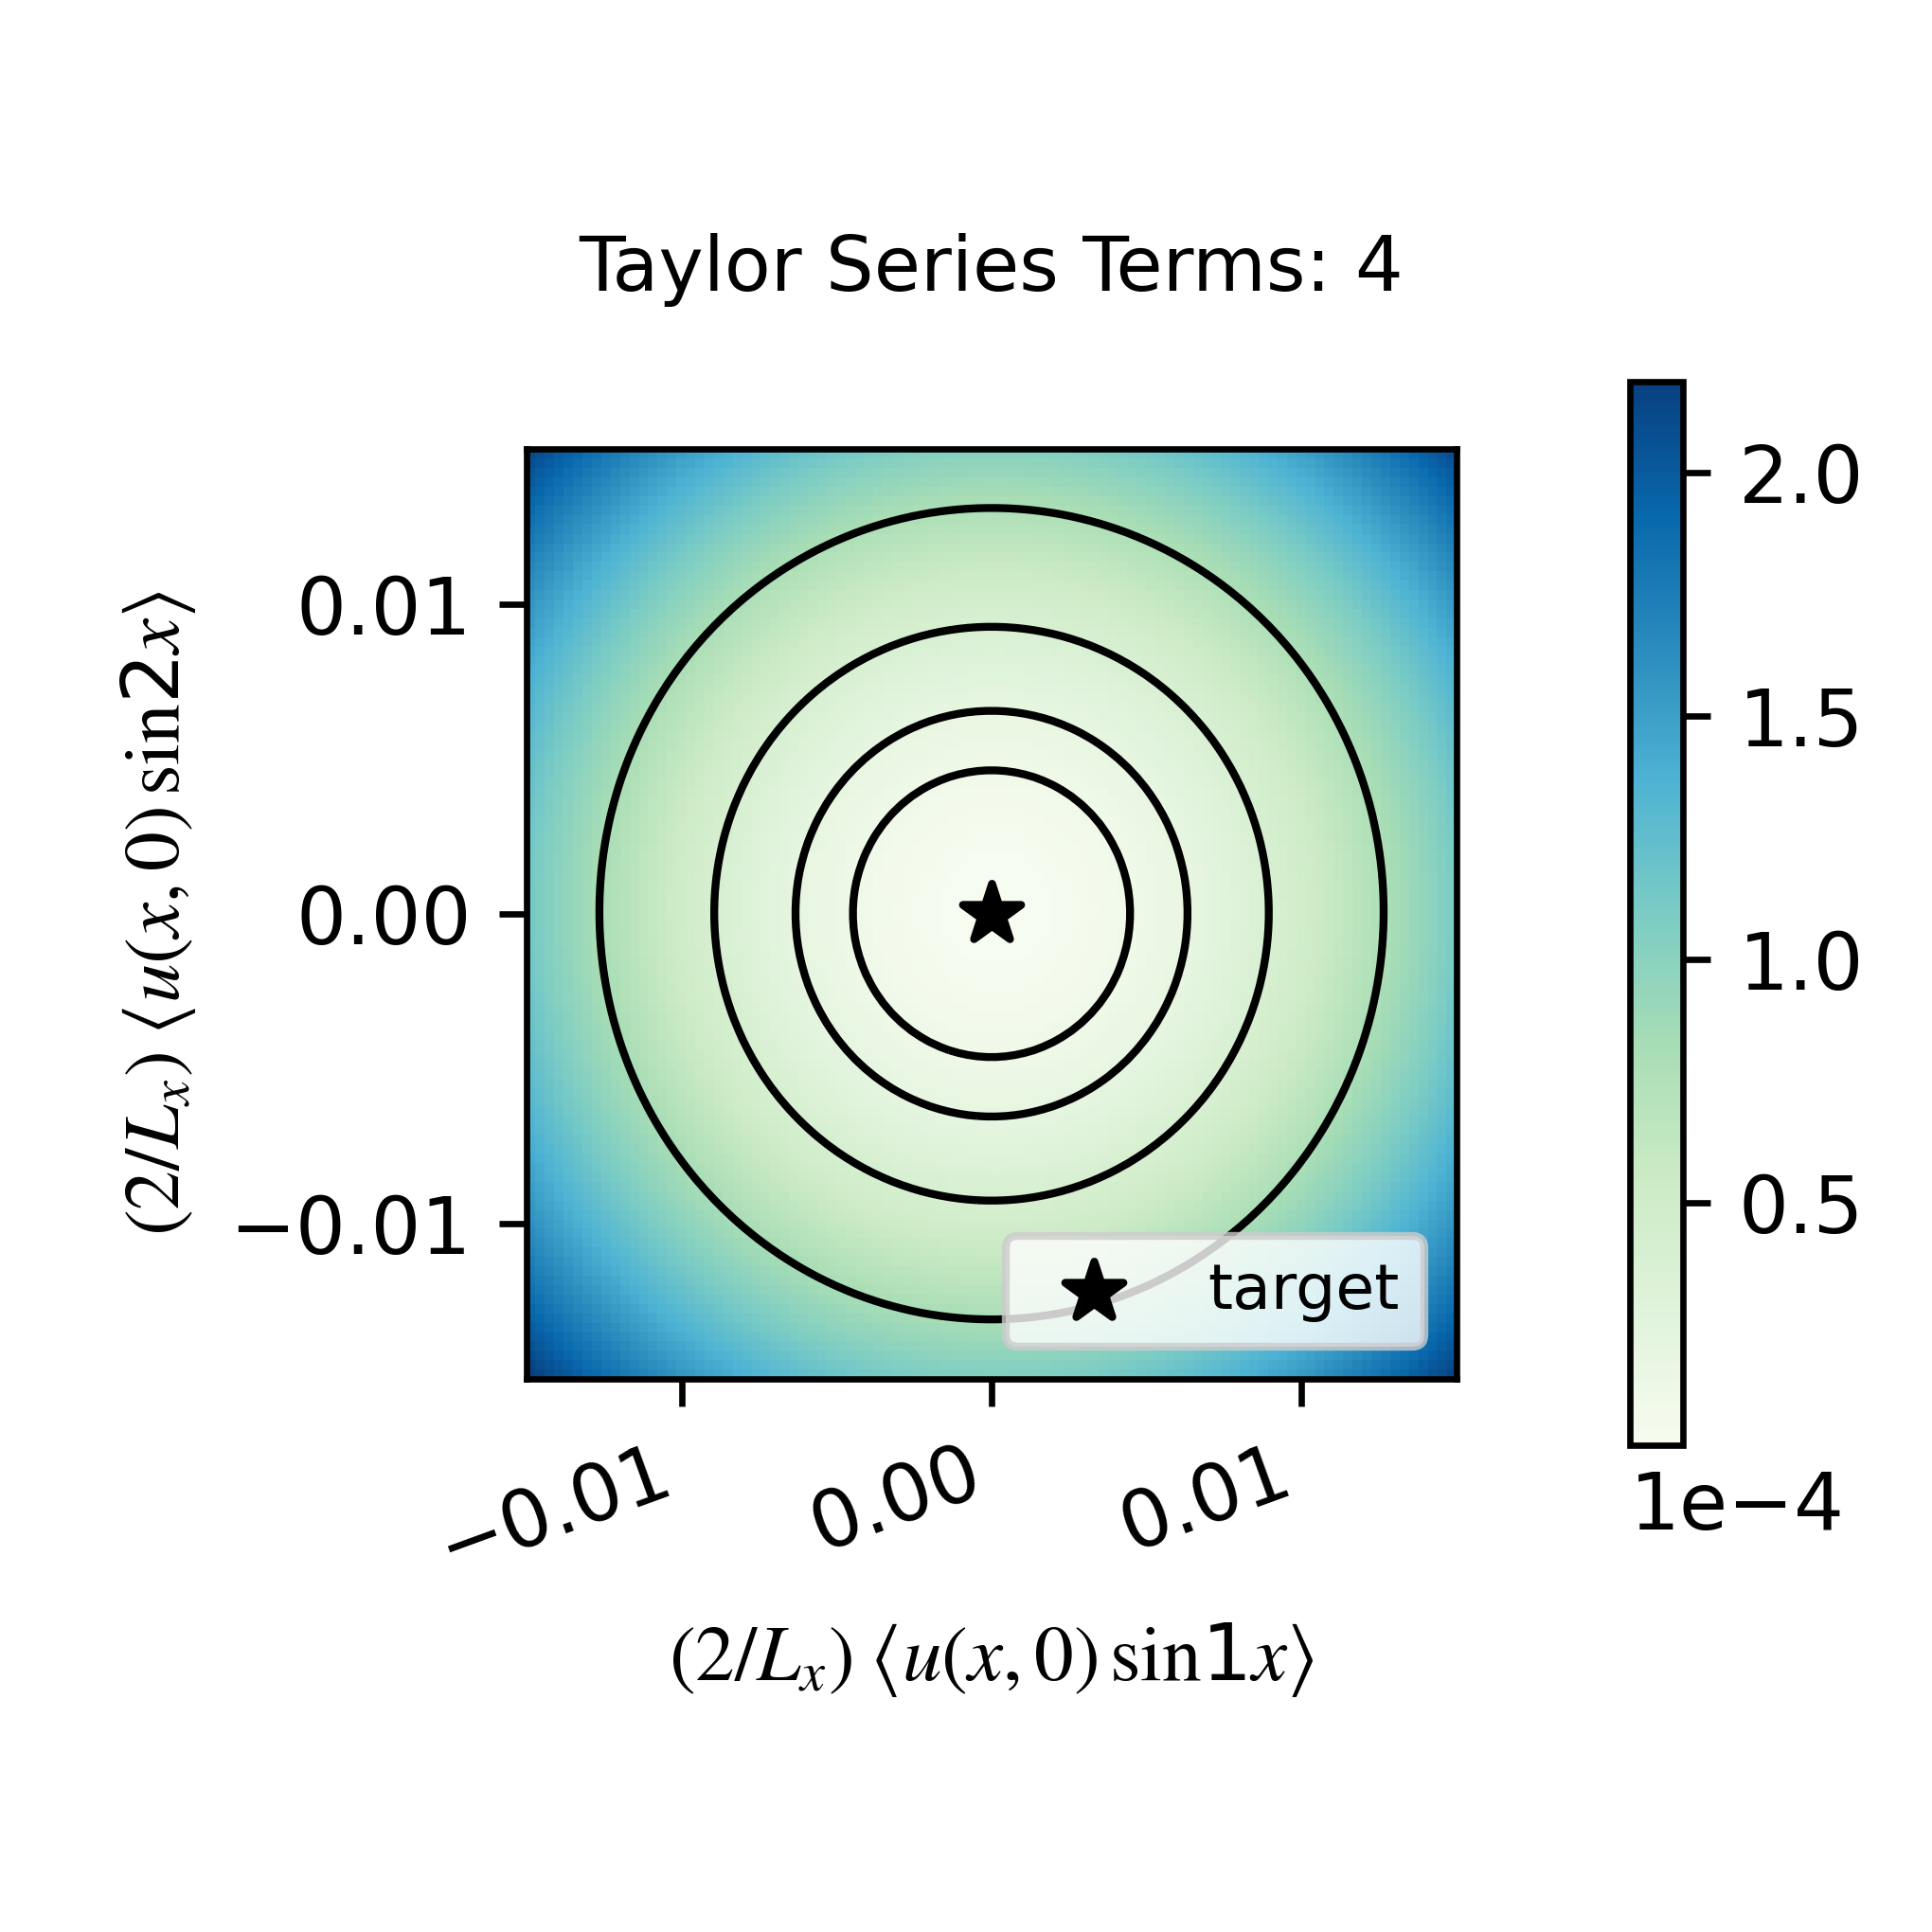
\includegraphics[width=3in]{SPHRtest_Nts4a0p3b0p0c0p0T1p0R0p015kt10p0kt20.png}
  \end{tabular}
  % \caption{Heat fluxes (left) and eigenvalue spectra (right) of equilibrated states with $\Ra = 2 \times 10^5$ (top) and $\Ra = 10^9$ (bottom). 
  % The heat flux profiles are symmetric about $z=0$, so we only plot for $z<0$.
  % We plot the advection profiles for marginally-stable modes. 
  % At low $\Ra$, a single mode with $k_x = 1.5\pi$ is sufficient to oppose boundary layer diffusion and facilitate heat flux throughout the bulk of the domain. 
  % At large $\Ra$, high-wavenumber modes contribute pronounced small-scale advection profiles which tightly hug the thin boundary layers. 
  % A combination of progressively wider advection profiles is necessary to transition to bulk advection provided by the $k_x = 1.5\pi$ mode. 
  % This bulk mode mimics the large-scale convective cells which are characteristic of Rayleigh–Bénard convection, both in qualitative structure and number of cells in the domain.
  % The eigenfunctions which compose the advective profiles are illustrated in Appendix~\ref{sec:eigenfunctions}.}
  % \label{fig:flux}
\end{figure*}

\clearpage
When the initial deviation $u'(x, 0)$ is described using a basis of fourier coefficients, its levelsets form hyperellipses, whose semi-major (semi-minor) axes are aligned with $u'(x, 0)$'s largest (smallest) fourier coefficient.
Accordingly, the path of steepest descent is only aligned with $u'(x, 0)$ when $u'(x, 0)$ is composed of a single fourier mode. Such systems are self-adjoint, meaning $L[u] = L^{\dagger}[u]$

% \begin{figure}
%   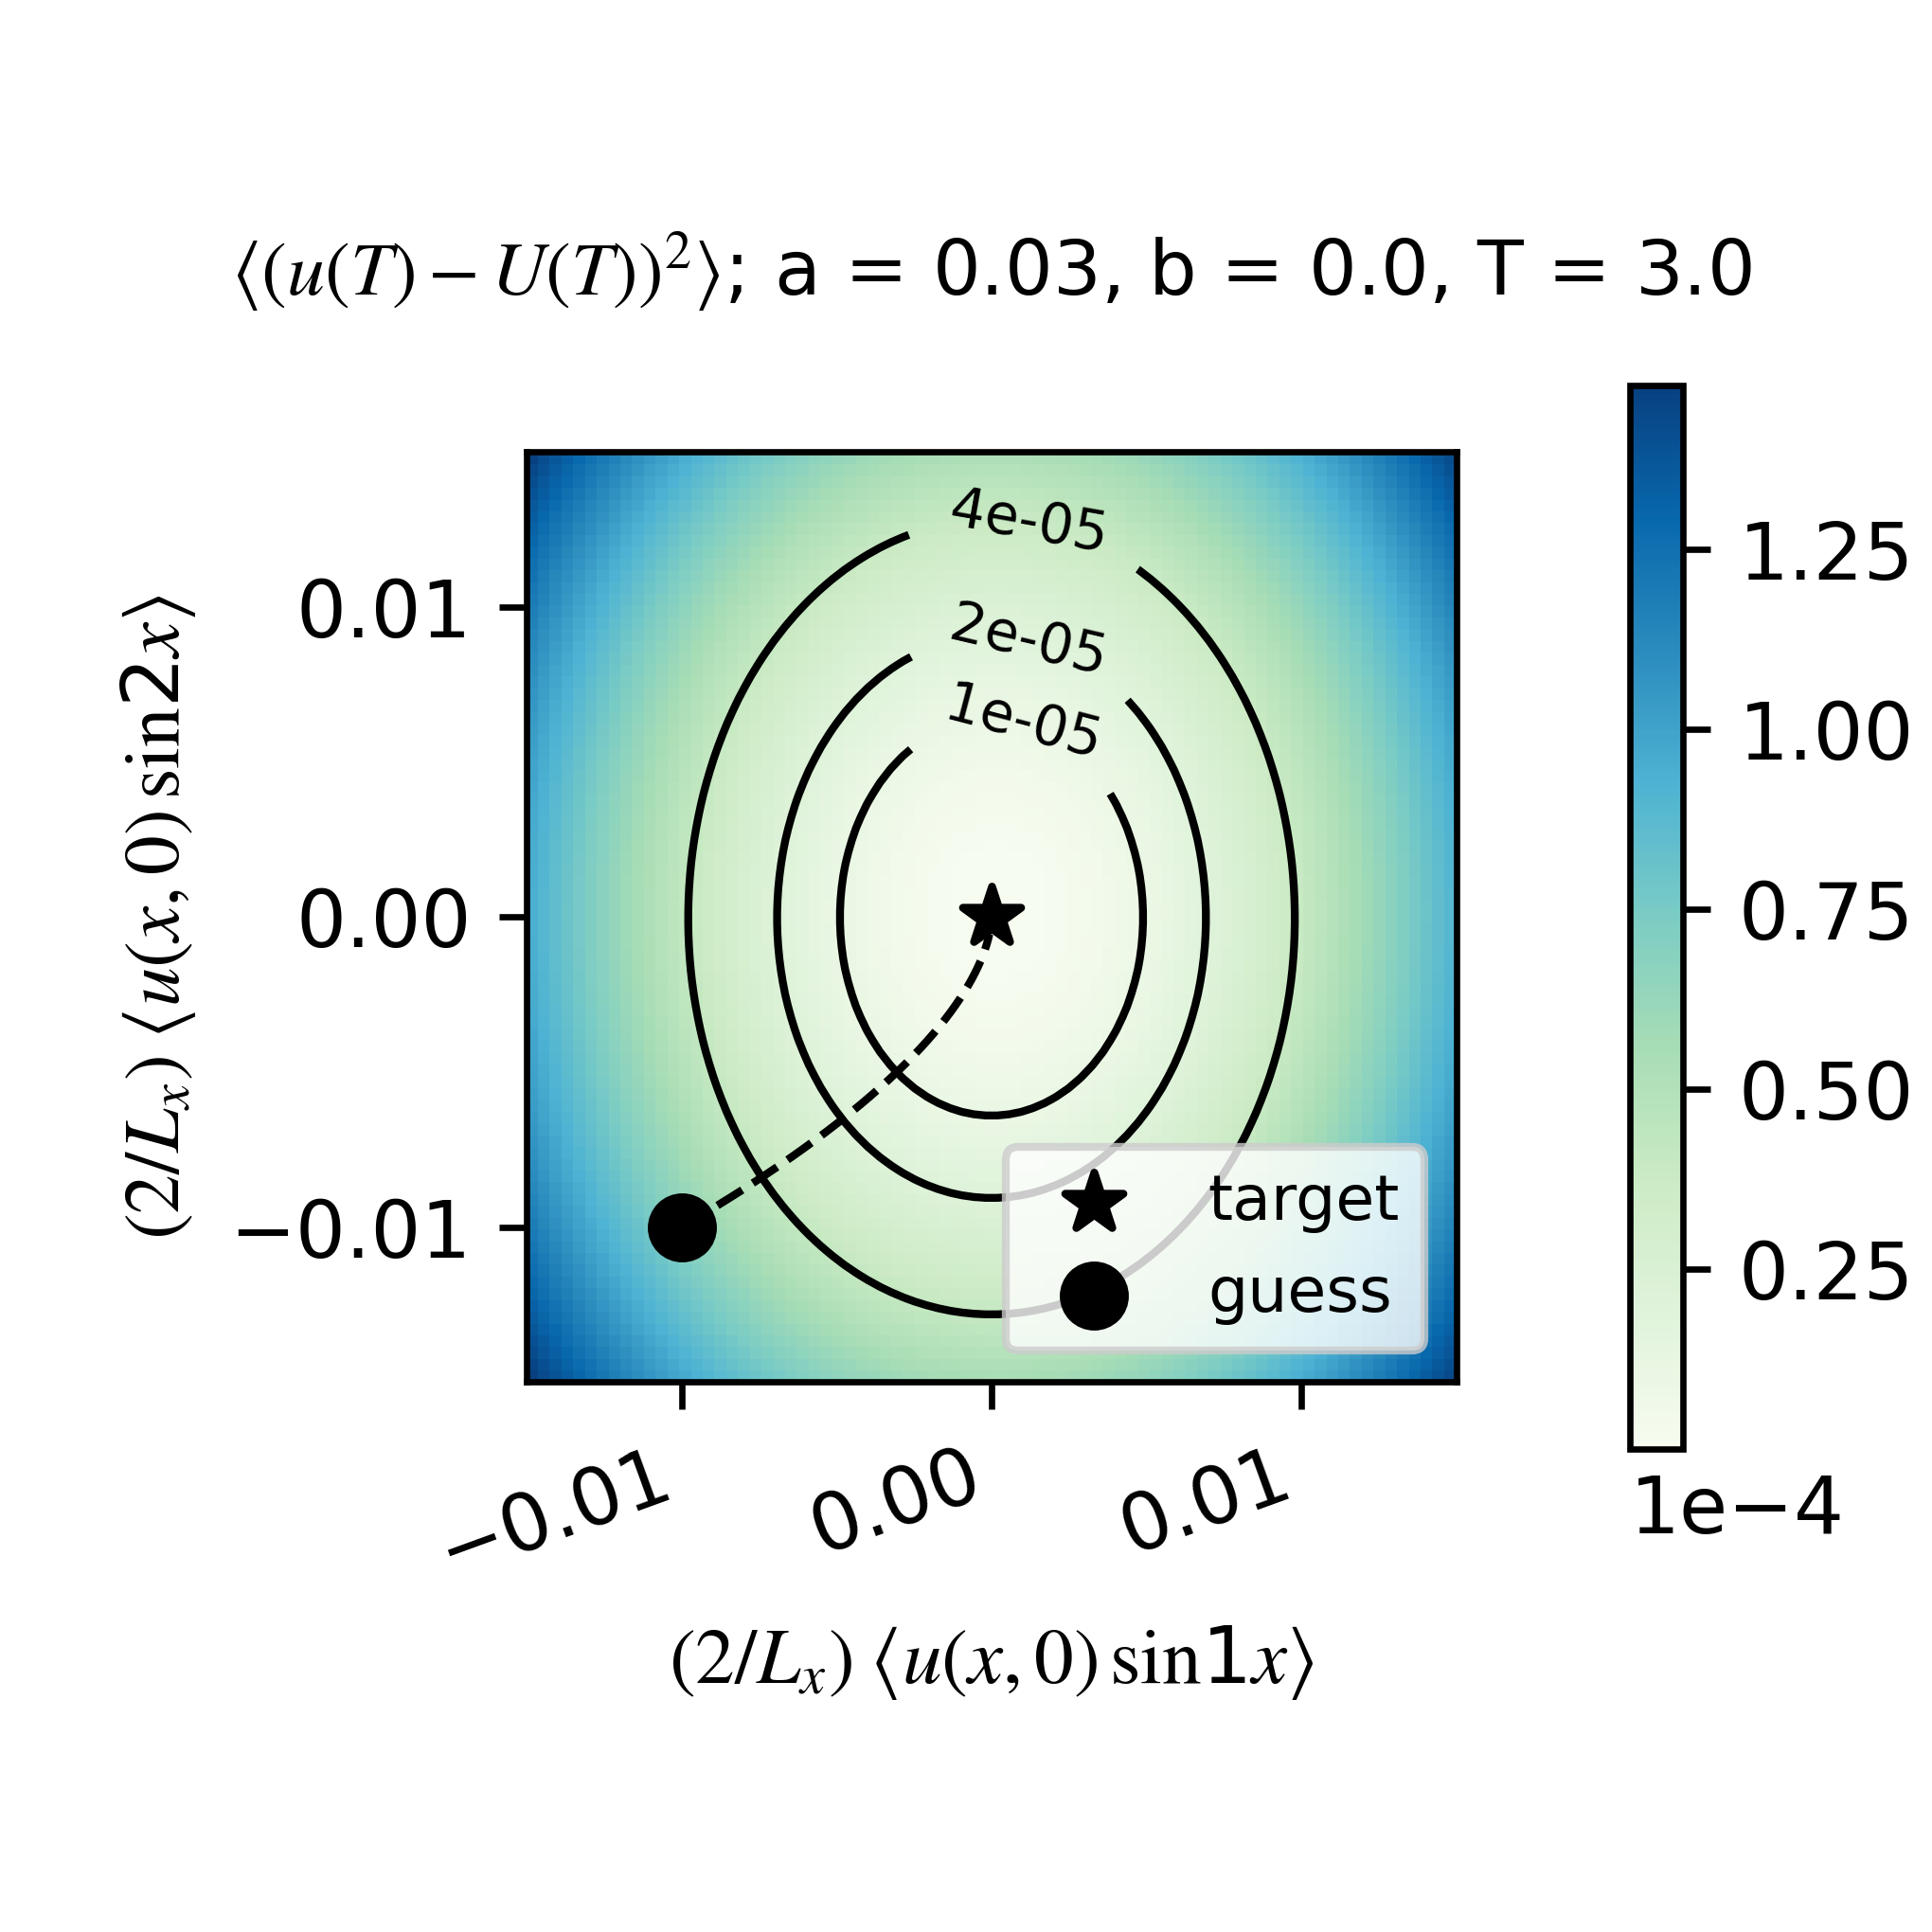
\includegraphics[width=9cm]{objtest_a0p03b0p0c0p0T3p0R0p015kt10p0kt20.png}
%   \caption{Objective function and an example gradient descent path for the diffusion equation. The target simulation $U(t) = 0$ and the deviation is composed of two fourier modes, i.e. $u'(t) = a_1\sin x + a_5\sin 5x$. Because the system is linear self-adjoint, each subsequent guess in the gradient descent trajectory is constrained to lie in this 2D phase space.}
% \end{figure}

\textbf{summary: }Linear systems' objective functions' shapes do not depend on the target--the target manifests itself as a constant shift in ic space. 
Reversible wave equations, which conserve energy yield objective functions whose levelsets in ic space are spherical, so the gradient at any given guess always provides the shortest path to the target. 
In contrast, irreversible diffusive terms distort the spherical levelsets into hyperellipses, whose semi-minimum (maximum) axis is oriented in the direction of the lowest (highest) wavenumber fourier mode's coefficient.
Thus, when traversing an arbitrary path of steepest descent toward the target IC, low wavenumber modes are matched with the target first, followed by increasingly higher wavenumber modes.
\clearpage
\subsection{Nonlinear Reversible Problems}
Here the target matters. We consider burger's equation
\begin{align*}
  \partial_t u + u\partial_x u &= b \, \partial_x^3 u
  \intertext{where energy is conserved}
  0 &= \partial_t \langle \frac{1}{2}u^2 \rangle + \langle u^2\partial_x u\rangle - b\davg{u\partial_x^3 u}\\
  &= \partial_t \langle \frac{1}{2}u^2 \rangle + \langle  \frac{1}{3}\partial_x u^3\rangle  \\
  &= \partial_t \langle \frac{1}{2}u^2 \rangle \\
  \\
  \partial_x^3 (u*u) &= 2\partial_x^2[ u\partial_x u ] \\
  &= 2\partial_x[ (\partial_x u)^2 + u\partial_x^2 u ]\\
  &= 2\partial_x[ (\partial_x u)^2] + \partial_x u\partial_x^2 u + u\partial_x^3 u \\
  &= \frac{5}{2} \partial_x[ (\partial_x u)^2] + u\partial_x^3 u \\
\end{align*}
Next we consider a guess with a known deviation from the target $u(x, 0) = U(x, 0) + u'(x, 0)$. Our objective function is given by $\langle (u(T) - U(T))^2 \rangle = \langle u'^2(T) \rangle$. The forward evolution equation for the perturbation is given by

\begin{align}
  0 &= \partial_t u' + u'\partial_x U + U\partial_x u' + u'\partial_x u' - b\partial_x^3 u'\label{pertbrg}\\
  \intertext{then we have that}
  \intertext{the evolution of the target is given by}
  0 &= \frac{1}{2}\partial_t \davg{u'^2} + \davg{u' \partial_x (u'U)} + \davg{\frac{1}{3}\partial_x u'^3} \nonumber \\
  &= \frac{1}{2}\partial_t \davg{u'^2} +  \davg{u' \partial_x (u'U)} \nonumber \\
  &= \frac{1}{2}\partial_t \davg{u'^2} - \frac{1}{2}\davg{U \partial_x (u'^2)} \nonumber \\
  &\therefore\nonumber\\
  \davg{u'^2(T)} &= \davg{u'^2(0)} + \int_0^T \davg{U \partial_x (u'^2)} dt \label{objburgeq}
  % \intertext{Suppose $u' = \alpha U$. In this case $u = U + u' = (1+\alpha)U$ evolves identically to $U$ but at a rate which is $(1 + \alpha)^2$ faster. Thus the objective is given by $\davg{(U((1+\alpha)^2 T) - U(T))^2}$}.
  % % \intertext{Suppose the perturbation is small enough that its nonlinear term can be neglected. In this case we find that}
  % u'(T) &= u'(0) + \int_0^T \partial_tu'dt \\
  % &= u'(0)-\int_0^T \partial_x (u'U) + \frac{1}{2}\partial_x (u'^2) dt
  % \intertext{Therefore $\davg{u'(T)} = \davg{u'(0)}$. The objective function}
  % \davg{u'(T)^2}&= \davg{u'(0)^2}- \davg{u'(0)\int_0^T \partial_x (u'U) + \frac{1}{2}\partial_x (u'^2) dt} \\
  % &\;\; + \davg{\Big[\int_0^T \partial_x (u'U) + \frac{1}{2}\partial_x (u'^2) dt\Big]^2} \\
\end{align}

\subsection*{Numerical Examples}
Suppose the target solution is $U(t) = 0$. Then the perturbation equation (\ref{pertbrg}) is linear in $u'$, and we revert back to the hyperspherical levelsets described for wave equations in the previous section, as shown in Fig \ref{brgU0}.

\begin{figure}[H]
  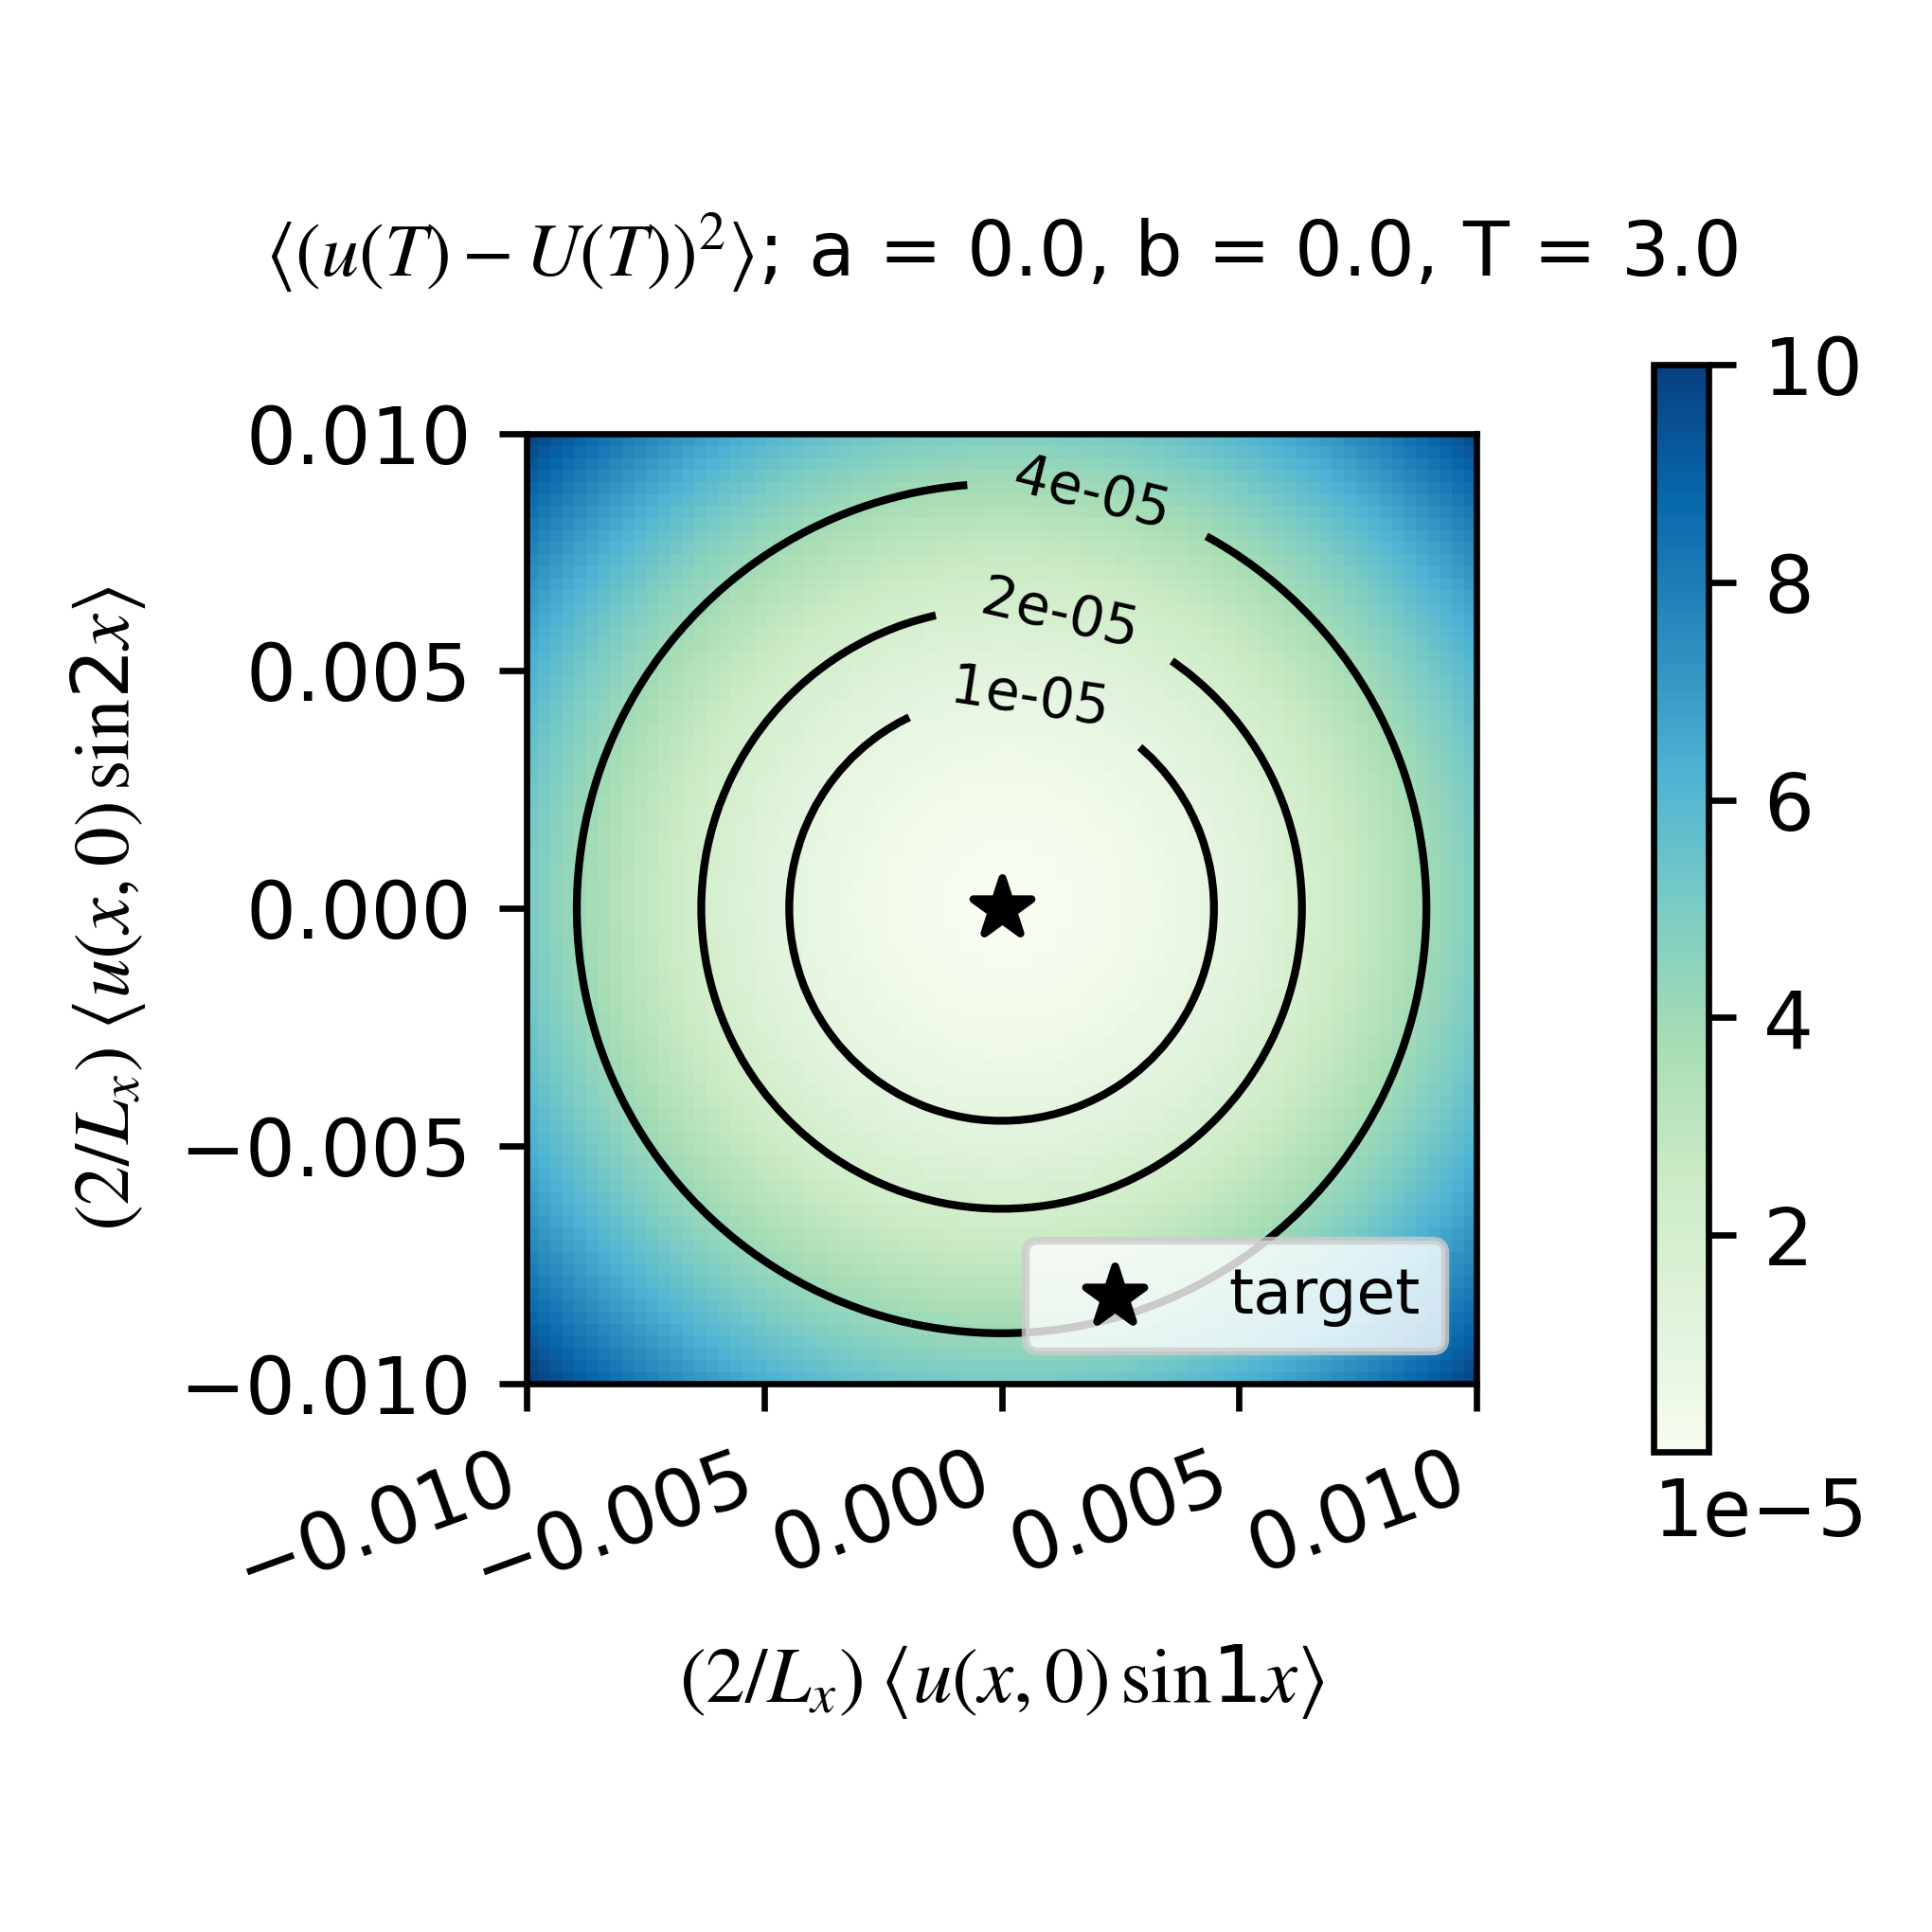
\includegraphics[width=9cm]{objtest_a0p0b0p0T3p0R0p01kt10p0kt20.png}
  % 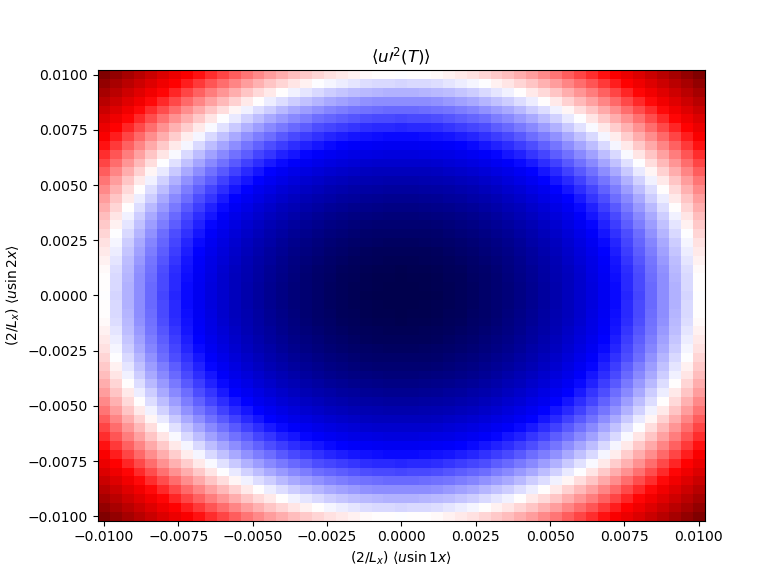
\includegraphics[width=9cm]{../diffusion/burgobjtest_k1k2_U0.png}
  \caption{Objective functional the inviscid burger's equation. The target simulation $U(x, 0) = 0$ and the deviation is composed of two fourier modes, i.e. $u'(t) = a_1\sin x + a_5\sin 2x$. Gradient descent paths will not deviate from this 2D phase space because the path of steepest descent is always in the radial direction.}
  \label{brgU0}
\end{figure}

Suppose instead that our target initial condition is given by $U(x, 0) = 5\sin(x)$ and we are interested in the 2D phase space of initial deviations $u'(x, 0) = a_1\sin x + a_2 \sin 2x$, as shown in Fig \ref{brgU5m1}.. 

\begin{figure}[H]
  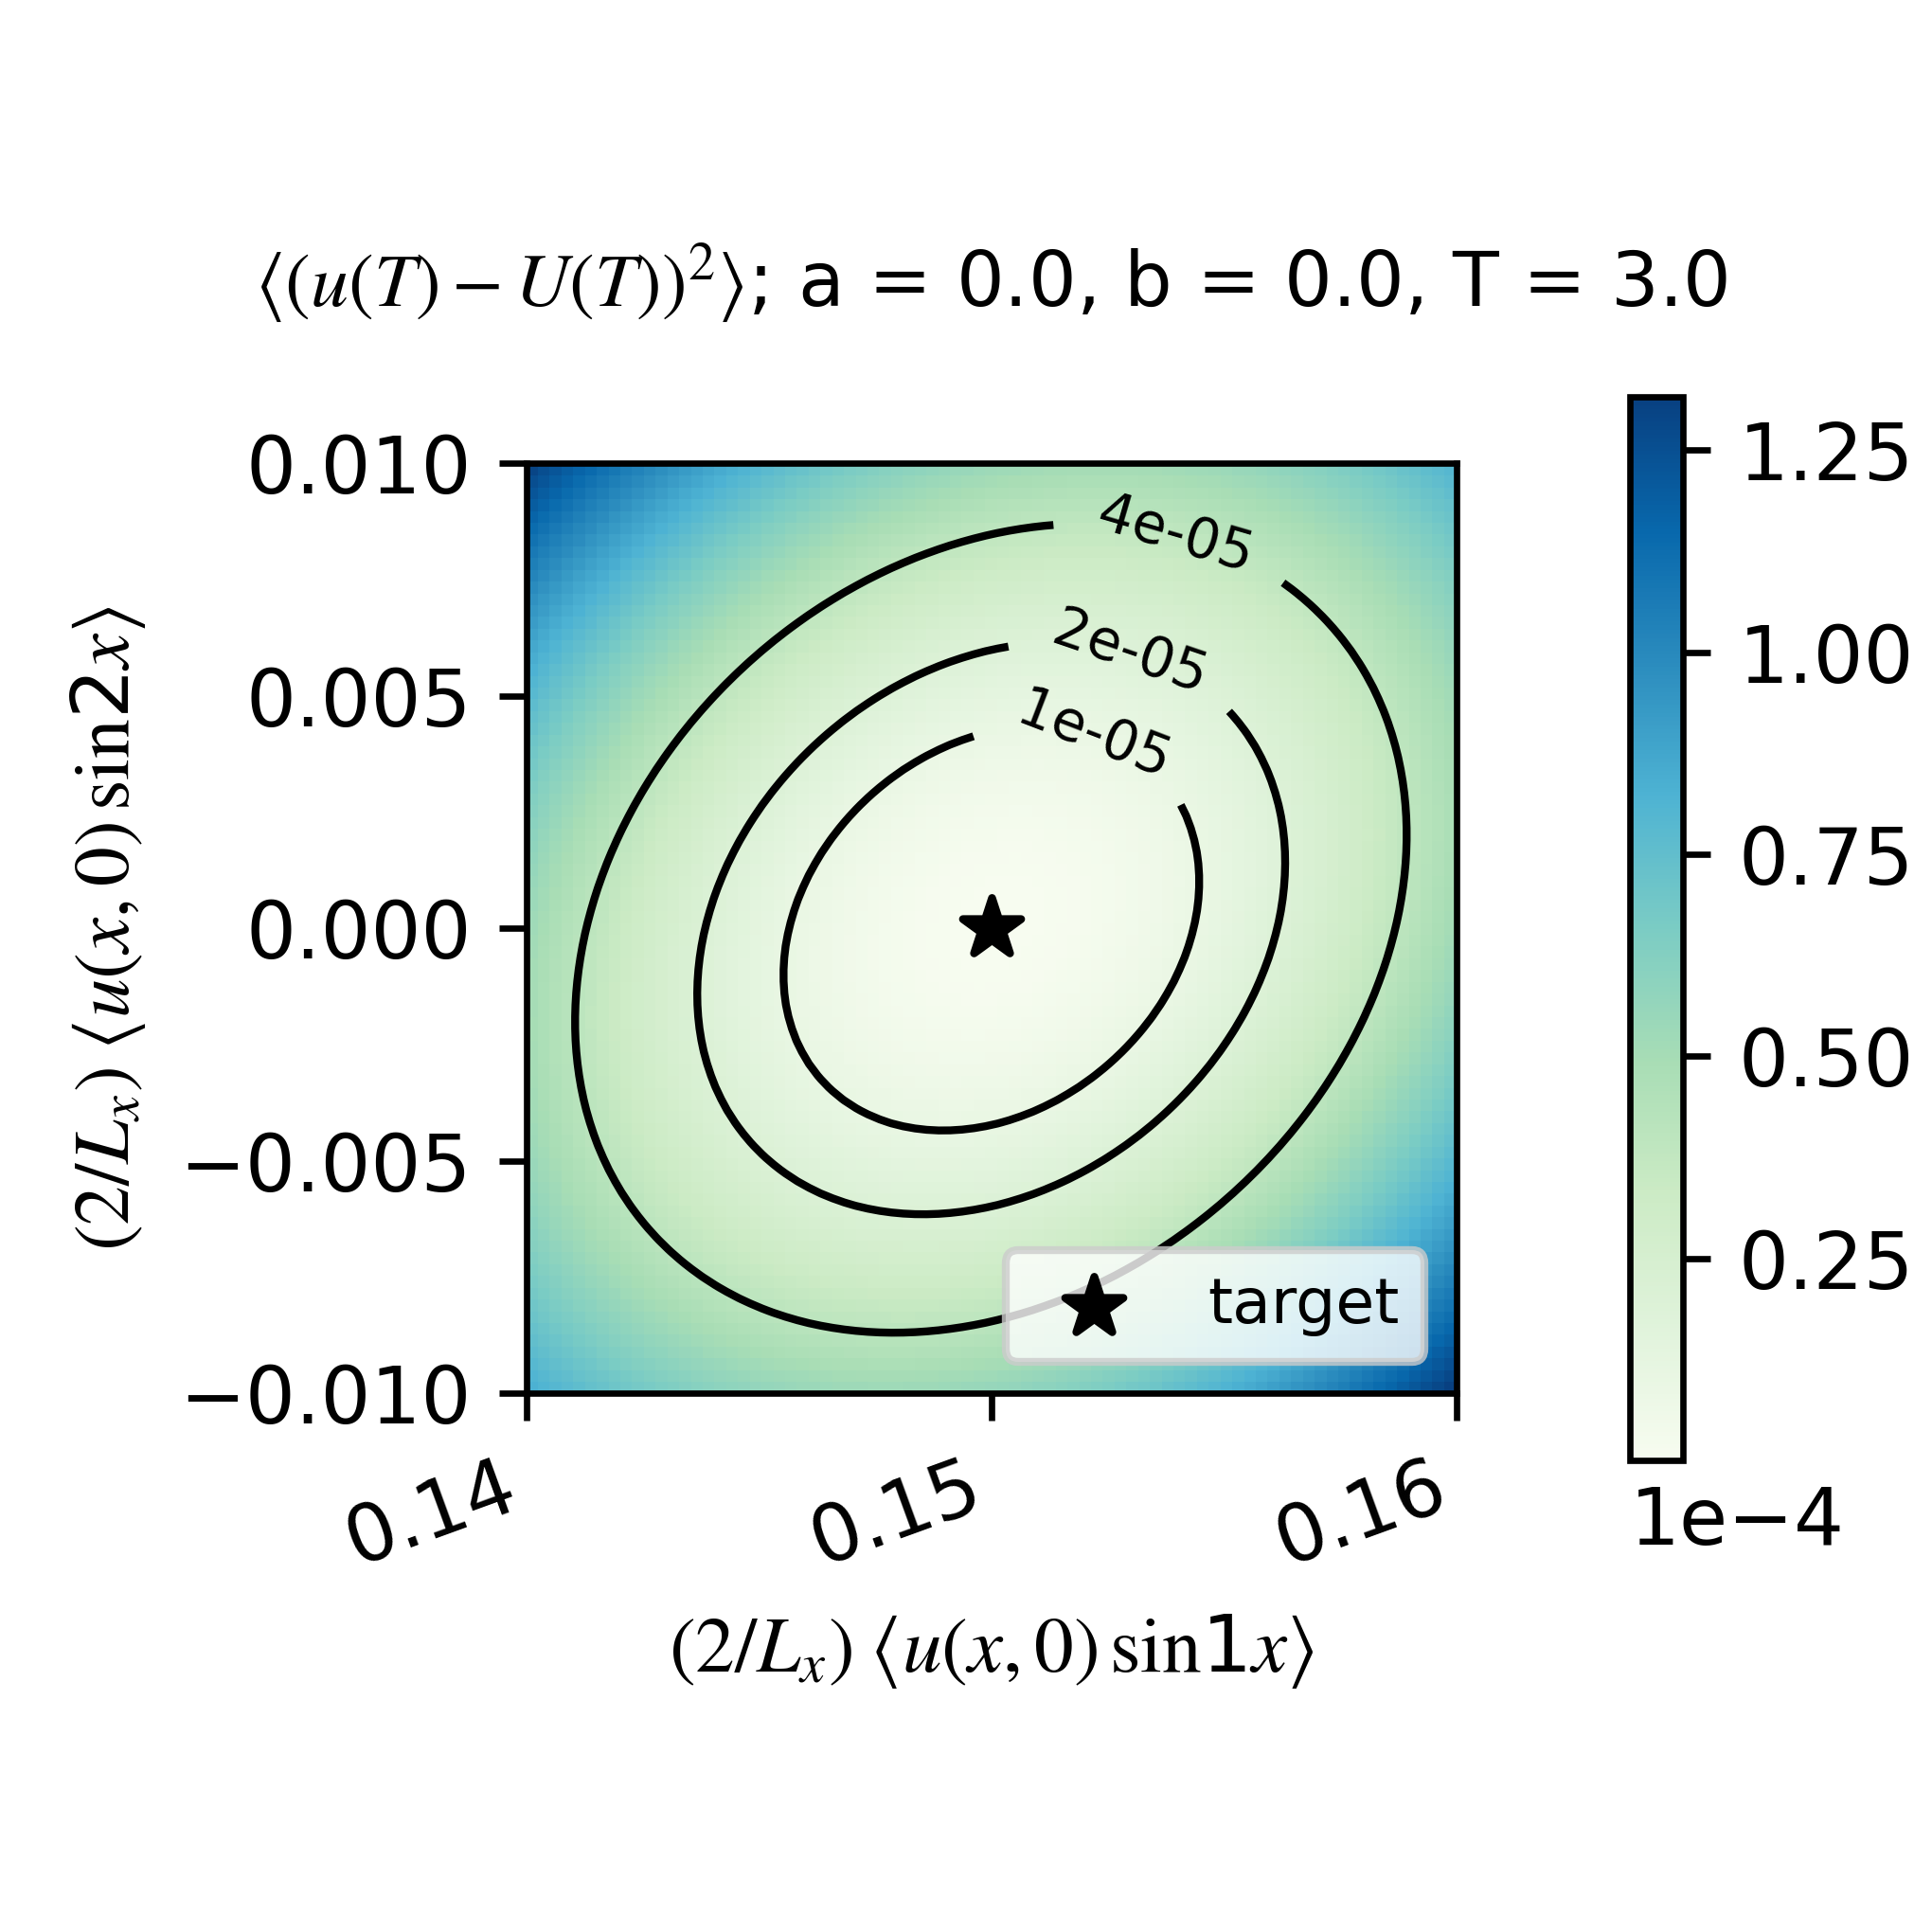
\includegraphics[width=9cm]{objtest_a0p0b0p0T3p0R0p01kt10p15kt20.png}
  \caption{Objective functional the inviscid burger's equation. The target simulation $U(x, 0) = 5\sin x$ and the deviation is composed of two fourier modes, i.e. $u'(t) = a_1\sin x + a_5\sin 2x$. Gradient descent paths will deviate from this 2D phase space because external fourier modes are populated by the nonlinearities in the forward and adjoint equations.}
  \label{brgU5m1}
\end{figure}


\clearpage
\bibliography{lsrtm.bib}

\end{document}
